
%% The vignette is build automatically with the package
%% You can build the vignette also on its own. 
%% I (Markus) use the devtools package by Hadley Wickham to do this:
%% library(devtools)
%% build_vignettes("~/Dropbox/chainladder")

\documentclass{article}
\usepackage[T1]{fontenc} 
\usepackage{Sweave}
\usepackage{thumbpdf}
\usepackage{url}
\usepackage{wrapfig}
\usepackage{hyperref}

\hypersetup{
  colorlinks=true,
  pdftitle={ChainLadder: Claims reserving with R},%
  pdfauthor={Markus Gesmann}%, Dan Murphy, Wayne Zhang},%
}

%\VignetteIndexEntry{ChainLadder: Claims reserving with R}




%\keywords{Claims, reserving, IBNR, chain ladder, 
%stochastic reserving, statistical software, \proglang{R}}

\setlength{\parindent}{0.0in}
\setlength{\parskip}{2mm}

\newcommand{\chainladder}{\textbf{\texttt{ChainLadder}} }
% Change default font to a sans serifs
\renewcommand{\familydefault}{\sfdefault}

\begin{document}

\author{Markus
  Gesmann\footnote{\href{mailto:markus.gesmann@gmail.com}{markus.gesmann@gmail.com}}
  %, Dan  Murphy\footnote{\href{mailto:danielmarkmurphy@gmail.com}{danielmarkmurphy@gmail.com}} 
  % and 
  % Wayne Zhang\footnote{\href{mailto:actuary\_zhang@hotmail.com}{actuary\_zhang@hotmail.com}} 
}

\title{Claims reserving with R:\\
  ChainLadder-0.1.5-2
  Package Vignette 
}
\maketitle
\begin{abstract}
  The \chainladder package provides various statistical methods which
  are typically used for the calculation of outstanding claims reserves
  in general insurance.  
  
  The package has implementations of the Mack-, Munich-, Bootstrap, and
  multi-variate chain-ladder methods, as well as the loss development
  factor curve fitting methods of Dave Clark and generalised linear
  model based reserving models. 
\end{abstract}

\clearpage
\tableofcontents
\clearpage

\section{Introduction}

\subsection{Claims reserving in insurance}
Unlike other industries the insurance industry does not sell products
as such, but promises. An insurance policy is a promise by the insurer
to the policyholder to pay for future claims for an upfront received
premium. 

As a result insurers don't know the upfront cost of their
service, but rely on data analysis and judgement to derive a
sustainable price for their offering. In General Insurance (or Non-Life
Insurance) most policies run for a period of 12 months, e.g. motor,
property and casualty insurance. However, the claims payment process
can take years or even decades. 

In particular claims arising from casualty insurance can take a long
time to settle, as claims can take years to materialise. A complex and
costly example are the claims from asbestos liabilities. 
A research report by a  Working Party of the  Institute of Actuaries
has estimated that the undiscounted cost of UK mesothelioma-related
claims to the UK Insurance Market for the period 2009 to 2050 could be
around $\pounds$10bn~\cite{Gravelsons2009}. The cost for Asbestos
related claims in the US for the worldwide insurance industry was
estimate to be around \$120bn in 2002~\cite{Michaels2002}.  

Thus, it should come to no surprise that the biggest item on the
liability side of an insurer's balance sheet is often the provision or
reserves for future claims payments. Those reserves can be broken
down in case reserves (or out-standings claims), which are losses
already reported to the insurance company and incurred but not
reported (IBNR) claims.

Over the years several methods have been developed to estimate
reserves for insurance claims, see~\cite{Schmidt2011},
\cite{EnglandVerrall2002} for an overview. Changes in the regulatory
requirements, e.g. Solvency II\footnote{See
  \url{http://ec.europa.eu/internal_market/insurance/solvency/index_en.htm}}
in Europe, have fostered further research into this topic, with a
focus on stochastic and statistical techniques.   

\section{The \chainladder package}

\subsection{Motivation}
The \chainladder~\cite{chainladder} package provides various
statistical methods which are typically used for the calculation of
outstanding claims reserves in general insurance.  The package started
out of presentations given by Markus Gesmann at the Stochastic
Reserving Seminar at the Institute of Actuaries in 2007 and 2008,
followed by talks at Casualty Actuarial Society (CAS)  meetings joined
by Dan Murphy in 2008 and Wayne Zhang in 2010.  

Implementing reserving methods in R has several advantages, as it provides:

\begin{itemize}

\item Rich language for statistical modelling and data manipulations
  allowing fast prototyping  
  
\item Very active user base, which publishes many extension
 
\item Many interfaces to data bases and other applications, such as MS
  Excel
  
\item Established framework for documentation and testing 

\item Works well with existing tools for version control 

\item Code is written in plain text files, allowing effective knowledge
  transfer 

\item Easy to collaborate over the internet

\item Built in functions to create reproducible research
  reports\footnote{For an example see the project: Formatted Actuarial Vignettes in
    R, \url{http://www.favir.net/}}

\item In combination with other tools such as  {\LaTeX} and Sweave
  easy to set up automated reporting

\item Academic research often first available in R  
    
\end{itemize}


\subsection{Brief package overview}
This vignette will give the reader a brief overview of the functionallity of 
the \chainladder package. The functions are discussed and explained in 
more detail in the repective help files and examples. The help files contain 
also the reference to the research papers on which the methods are based. 

The \chainladder package has implementations of the Mack-, Munich- and 
Boot\-strap chain-ladder methods~\cite{Mack1993}, \cite{Mack1999}, 
\cite{Quarg2004}, \cite{EnglandVerrall1999}. 
Since version 0.1.3-3 it provides general multivariate 
chain ladder models by Wayne Zhang~\cite{Zhang2010a}. 

Version 0.1.4-0 introduced new functions on loss development factor
(LDF) fitting and Cape Cod by Daniel Murphy following a paper by David
Clark~\cite{Clark2003}.  Version 0.1.5-0 has added loss reserving
models within the generalized linear model framework following a paper by
England and Verrall~\cite{EnglandVerrall1999} implemented by Wayne
Zhang.  

The package offers also some utility functions to convert quickly
tables into triangles, triangles into tables, cumulative into
incremental and incremental into cumulative triangles. 

Further, the \chainladder package comes with an example spreadsheet which
demonstrates how to use the \chainladder functions in Excel with
RExcel~\cite{rexcel}. The  spreadsheet is located in the Excel folder
of the package. The R command 
\begin{Schunk}
\begin{Sinput}
R> system.file("Excel", package="ChainLadder") 
\end{Sinput}
\end{Schunk}
will tell you the exact path to the directory. To use the spreadsheet you will need the
RExcel-Add-in~\cite{BaierNeuwirth2007}. The package also provides an
example SWord~\cite{BaierNeuwirth2007} file,  demonstrating how the
the functions of the package can be integrated into a MS Word file via
SWord. Again you find the Word file via the command: 
\begin{Schunk}
\begin{Sinput}
R> system.file("SWord", package="ChainLadder") 
\end{Sinput}
\end{Schunk}

The package comes with several demos to provide you with an overview
of the package functionality, see
\begin{Schunk}
\begin{Sinput}
R> demo(package="ChainLadder")
\end{Sinput}
\end{Schunk}
For more information and examples see the project web site:
\url{http://code.google.com/p/chainladder/}

\subsection{Installation}
We can install \chainladder in the usual way from CRAN, e.g.:
\begin{Schunk}
\begin{Sinput}
R> install.packages('ChainLadder') 
\end{Sinput}
\end{Schunk}
The installation was successful if the
command \texttt{library(ChainLadder)} gives you the following message:
\begin{Schunk}
\begin{Sinput}
R> library(ChainLadder)
\end{Sinput}
\end{Schunk}
\begin{Schunk}
\begin{Soutput}
ChainLadder version 0.1.5-2 by:
Markus Gesmann <markus.gesmann@gmail.com>
Wayne Zhang <actuary_zhang@hotmail.com>
Daniel Murphy <danielmarkmurphy@gmail.com>

Type library(help='ChainLadder') or ?ChainLadder
to see overall documentation.

Type demo(ChainLadder) to get an idea of the functionality of this package.

See demo(package='ChainLadder') for a list of more demos.

Feel free to send us an email if you would like to keep informed of
new versions or if you have any feedback, ideas, suggestions or would
like to collaborate.

More information is available on the ChainLadder project web-site:
http://code.google.com/p/chainladder/

To suppress this message use the statement:
suppressPackageStartupMessages(library(ChainLadder))
\end{Soutput}
\end{Schunk}

\section{Using the  \chainladder package}

\subsection{Working with triangles}

Historical insurance data is often presented in form of a triangle structure.
Most reserving methods of the \chainladder package expect triangles as 
input data sets with development periods along the columns and the origin 
period in rows. The package comes with several example triangles. 
The following R command will list them all:
\begin{Schunk}
\begin{Sinput}
R> require(ChainLadder)
R> data(package="ChainLadder")
\end{Sinput}
\end{Schunk}

Let's look at one example triangle more closely. The following triangle shows 
data from the Reinsurance Association of America (RAA):
\begin{Schunk}
\begin{Sinput}
R> ## Sample triangle
R> RAA
\end{Sinput}
\begin{Soutput}
      dev
origin    1     2     3     4     5     6     7     8     9    10
  1981 5012  8269 10907 11805 13539 16181 18009 18608 18662 18834
  1982  106  4285  5396 10666 13782 15599 15496 16169 16704    NA
  1983 3410  8992 13873 16141 18735 22214 22863 23466    NA    NA
  1984 5655 11555 15766 21266 23425 26083 27067    NA    NA    NA
  1985 1092  9565 15836 22169 25955 26180    NA    NA    NA    NA
  1986 1513  6445 11702 12935 15852    NA    NA    NA    NA    NA
  1987  557  4020 10946 12314    NA    NA    NA    NA    NA    NA
  1988 1351  6947 13112    NA    NA    NA    NA    NA    NA    NA
  1989 3133  5395    NA    NA    NA    NA    NA    NA    NA    NA
  1990 2063    NA    NA    NA    NA    NA    NA    NA    NA    NA
\end{Soutput}
\end{Schunk}

\subsubsection{Plotting triangles}
For data set of class \texttt{triangle} \chainladder provides
default plotting methods to give a graphical overview of the data:
\begin{Schunk}
\begin{Sinput}
R> plot(RAA)
\end{Sinput}
\end{Schunk}

\begin{figure}
  \centering
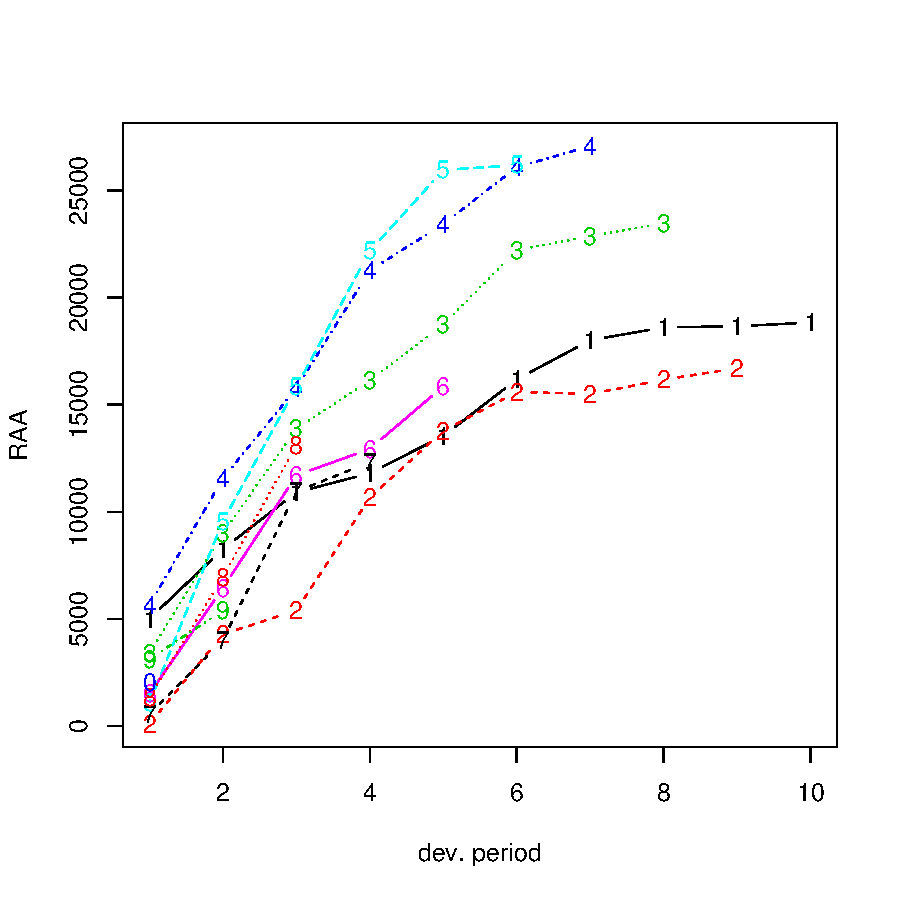
\includegraphics{ChainLadder-TrianglePlot1}
\caption{Claims development chart of the \texttt{RAA} triangle, with
  one line per origin period. Output of \texttt{plot(RAA)}
  }
\label{RAAplot}
\end{figure}

Setting the argument \texttt{lattice=TRUE} will produce individual
plots for each origin period\footnote{\chainladder uses the
  \href{http://cran.r-project.org/package=lattice}{\texttt{lattice}}
  package}, see Figure~\ref{RAAplot2}. 
\begin{Schunk}
\begin{Sinput}
R> plot(RAA, lattice=TRUE)
\end{Sinput}
\end{Schunk}

\begin{figure}
  \centering
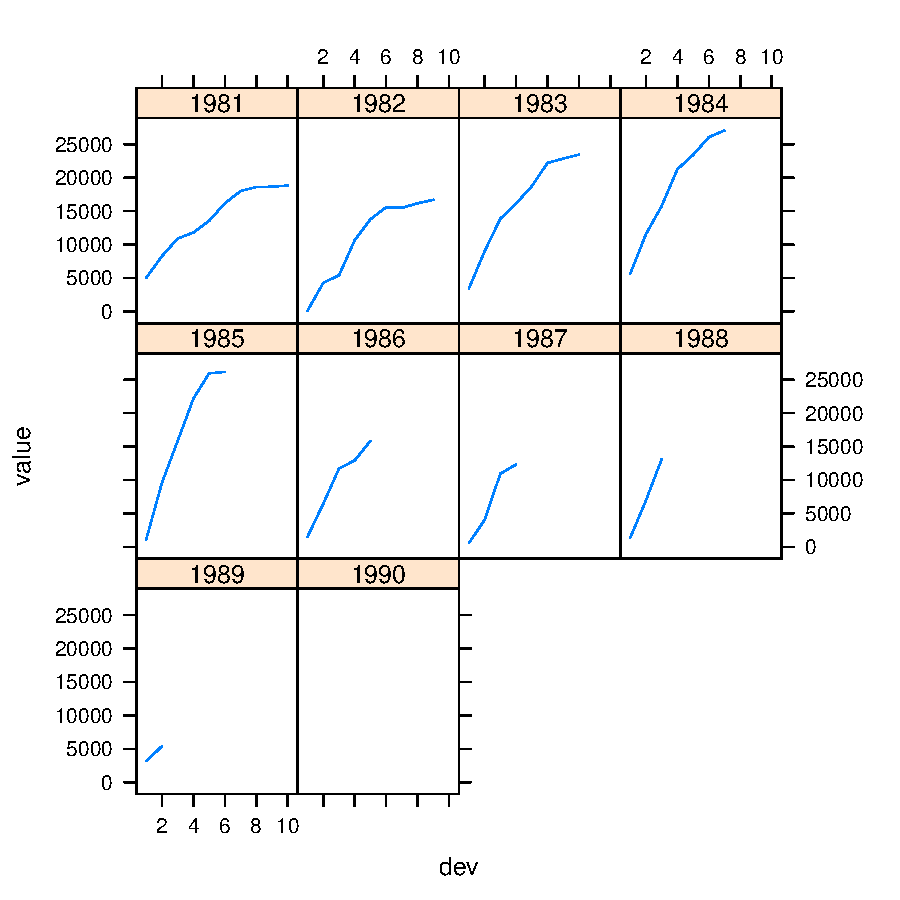
\includegraphics{ChainLadder-TrianglePlot2}
\caption{Claims development chart of the \texttt{RAA} triangle, with
  individual panels for each origin period. Output of
  \texttt{plot(RAA, lattice=TRUE)}
  }
\label{RAAplot2}
\end{figure}

You will notice from the plots in Figures~\ref{RAAplot},
\ref{RAAplot2}  that the triangle \texttt{RAA} present claims
developments for  the origin years 1981 to 1990 in a cumulative form.
For more information on the triangle plotting functions see the help
pages of \texttt{plot.triangle}, e.g. via
\begin{Schunk}
\begin{Sinput}
R> ?plot.triangle
\end{Sinput}
\end{Schunk}

\subsubsection{Transforming triangles between cumulative and
  incremental representation}
The \chainladder packages comes with two helper functions,
\texttt{cum2incr} and \texttt{incr2cum} to transform
cumulative triangles into incremental triangles and vis versa:
\begin{Schunk}
\begin{Sinput}
R> raa.inc <- cum2incr(RAA)
R> ## Show first origin period and its incremental development
R> raa.inc[1,]
\end{Sinput}
\begin{Soutput}
   1    2    3    4    5    6    7    8    9   10 
5012 3257 2638  898 1734 2642 1828  599   54  172 
\end{Soutput}
\begin{Sinput}
R> raa.cum <- incr2cum(raa.inc)
R> ## Show first origin period and its cumulative development
R> raa.cum[1,]
\end{Sinput}
\begin{Soutput}
    1     2     3     4     5     6     7     8     9    10 
 5012  8269 10907 11805 13539 16181 18009 18608 18662 18834 
\end{Soutput}
\end{Schunk}

\subsubsection{Importing triangles from external data sources}
In most cases you want to analyse your own data, usually stored in
data bases. R makes it easy to access data using SQL statements,
e.g. via an ODBC connection\footnote{See the
  \href{http://cran.r-project.org/package=RODBC}{\texttt{RODBC}}
  package} and the \chainladder packages includes a demo to showcase
how data can be imported from a MS Access data base, see: 
\begin{Schunk}
\begin{Sinput}
R> demo(DatabaseExamples)
\end{Sinput}
\end{Schunk}
For more details see~\cite{Rdata}.

In this section we use data stored in a CSV-file\footnote{Please
  ensure that your CSV-file is free from formatting, e.g. characters to
  separate units of thousands, as columns with those kind of
  formatting would be read as characters.} to demonstrate some
typical operations you will want to carry out with data stored in data bases.
In most cases your triangles will be stored in tables without the
classical triangle shape. The \chainladder packages contains a
CSV-file with some sample data in a long table format. We can read the
data into R's memory with the \texttt{read.csv} command and look at
the first couple of rows and summarise it:

\begin{Schunk}
\begin{Sinput}
R> filename <-  file.path(system.file("Database", 
+                                    package="ChainLadder"), 
+                        "TestData.csv")
R> myData <- read.csv(filename)
R> head(myData)
\end{Sinput}
\begin{Soutput}
  origin dev  value lob
1   1977   1 153638 ABC
2   1978   1 178536 ABC
3   1979   1 210172 ABC
4   1980   1 211448 ABC
5   1981   1 219810 ABC
6   1982   1 205654 ABC
\end{Soutput}
\begin{Sinput}
R> summary(myData)
\end{Sinput}
\begin{Soutput}
     origin          dev            value                         lob     
 Min.   :   1   Min.   : 1.00   Min.   : -17657   AutoLiab          :105  
 1st Qu.:   3   1st Qu.: 2.00   1st Qu.:  10324   GeneralLiab       :105  
 Median :   6   Median : 4.00   Median :  72468   M3IR5             :105  
 Mean   : 642   Mean   : 4.61   Mean   : 176632   ABC               : 66  
 3rd Qu.:1979   3rd Qu.: 7.00   3rd Qu.: 197716   CommercialAutoPaid: 55  
 Max.   :1991   Max.   :14.00   Max.   :3258646   GenIns            : 55  
                                                  (Other)           :210  
\end{Soutput}
\end{Schunk}
Let us focus on one subset of the data set. We select the RAA data again:
\begin{Schunk}
\begin{Sinput}
R> raa <- subset(myData, lob %in% "RAA")
R> head(raa)
\end{Sinput}
\begin{Soutput}
   origin dev value lob
67   1981   1  5012 RAA
68   1982   1   106 RAA
69   1983   1  3410 RAA
70   1984   1  5655 RAA
71   1985   1  1092 RAA
72   1986   1  1513 RAA
\end{Soutput}
\end{Schunk}
To transform the long table of the RAA data into a triangle we use the
function \texttt{as.triangle}. The arguments we have to specify are
the column names of the origin and development period and further the
column which contains the values:
\begin{Schunk}
\begin{Sinput}
R> raa.tri <- as.triangle(raa, origin="origin", dev="dev", value="value")
R> raa.tri
\end{Sinput}
\begin{Soutput}
      dev
origin    1    2    3    4    5    6    7   8   9  10
  1981 5012 3257 2638  898 1734 2642 1828 599  54 172
  1982  106 4179 1111 5270 3116 1817 -103 673 535  NA
  1983 3410 5582 4881 2268 2594 3479  649 603  NA  NA
  1984 5655 5900 4211 5500 2159 2658  984  NA  NA  NA
  1985 1092 8473 6271 6333 3786  225   NA  NA  NA  NA
  1986 1513 4932 5257 1233 2917   NA   NA  NA  NA  NA
  1987  557 3463 6926 1368   NA   NA   NA  NA  NA  NA
  1988 1351 5596 6165   NA   NA   NA   NA  NA  NA  NA
  1989 3133 2262   NA   NA   NA   NA   NA  NA  NA  NA
  1990 2063   NA   NA   NA   NA   NA   NA  NA  NA  NA
\end{Soutput}
\end{Schunk}
We note that the data has been stored as an incremental data set. As
mentioned above, we could now use the function \texttt{incr2cum} to
transform the triangle into a cumulative format.

We can transform a triangle back into a data frame structure:
\begin{Schunk}
\begin{Sinput}
R> raa.df <- as.data.frame(raa.tri, na.rm=TRUE)
R> head(raa.df)
\end{Sinput}
\begin{Soutput}
       origin dev value
1981-1   1981   1  5012
1982-1   1982   1   106
1983-1   1983   1  3410
1984-1   1984   1  5655
1985-1   1985   1  1092
1986-1   1986   1  1513
\end{Soutput}
\end{Schunk}

\subsubsection{Coping and pasting from MS Excel}
Small datas set in Excel can be transfered to R backwards and forwards
with via the clipboard under MS Windows.
\paragraph{Copying from Excel to R}
Select a data set in Excel and copy it into the clipboard, then go to
R and type:
\begin{Schunk}
\begin{Sinput}
R> x <- read.table(file="clipboard", sep="\t", na.strings="")
\end{Sinput}
\end{Schunk}
\paragraph{Copying from R to Excel}
Suppose you would like to copy the \texttt{RAA} triangle into Excel,
then the following statement would copy the data into the clipboard:
\begin{Schunk}
\begin{Sinput}
R> write.table(RAA, file="clipboard", sep="\t", na="")
\end{Sinput}
\end{Schunk}
Now you can paste the content into Excel. Please note that you can not
copy lists structures from R to Excel. 

\subsection{Chain-ladder methods}
\begin{Schunk}
\begin{Sinput}
R> demo(ChainLadder)
\end{Sinput}
\end{Schunk}
\subsubsection{Mack chain-ladder}
\begin{Schunk}
\begin{Sinput}
R> mack <- MackChainLadder(RAA, est.sigma="Mack")
R> mack
\end{Sinput}
\begin{Soutput}
MackChainLadder(Triangle = RAA, est.sigma = "Mack")

     Latest Dev.To.Date Ultimate   IBNR Mack.S.E CV(IBNR)
1981 18,834       1.000   18,834      0        0      NaN
1982 16,704       0.991   16,858    154      206    1.339
1983 23,466       0.974   24,083    617      623    1.010
1984 27,067       0.943   28,703  1,636      747    0.457
1985 26,180       0.905   28,927  2,747    1,469    0.535
1986 15,852       0.813   19,501  3,649    2,002    0.549
1987 12,314       0.694   17,749  5,435    2,209    0.406
1988 13,112       0.546   24,019 10,907    5,358    0.491
1989  5,395       0.336   16,045 10,650    6,333    0.595
1990  2,063       0.112   18,402 16,339   24,566    1.503

               Totals
Latest:    160,987.00
Dev:             0.76
Ultimate:  213,122.23
IBNR:       52,135.23
Mack S.E.:  26,909.01
CV(IBNR):        0.52
\end{Soutput}
\end{Schunk}

\begin{center}
\begin{Schunk}
\begin{Sinput}
R> plot(mack)
\end{Sinput}
\end{Schunk}
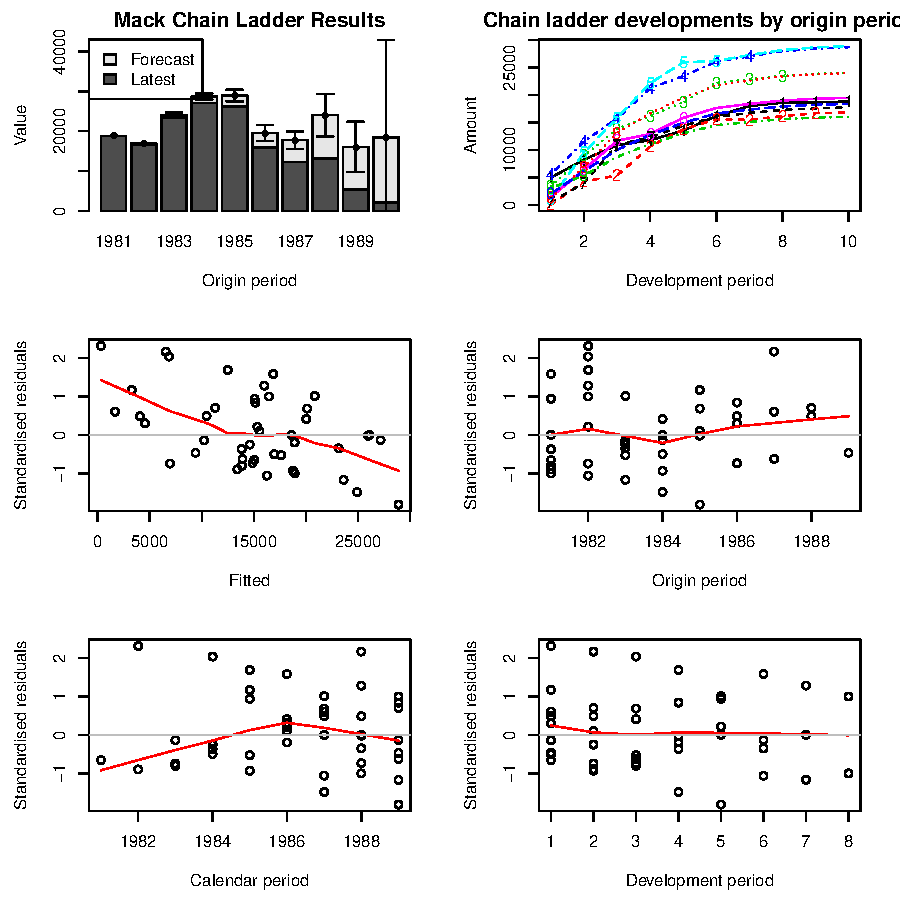
\includegraphics{ChainLadder-MackPlot1}
\end{center}

\begin{center}
\begin{Schunk}
\begin{Sinput}
R> plot(mack, lattice=TRUE)
\end{Sinput}
\end{Schunk}
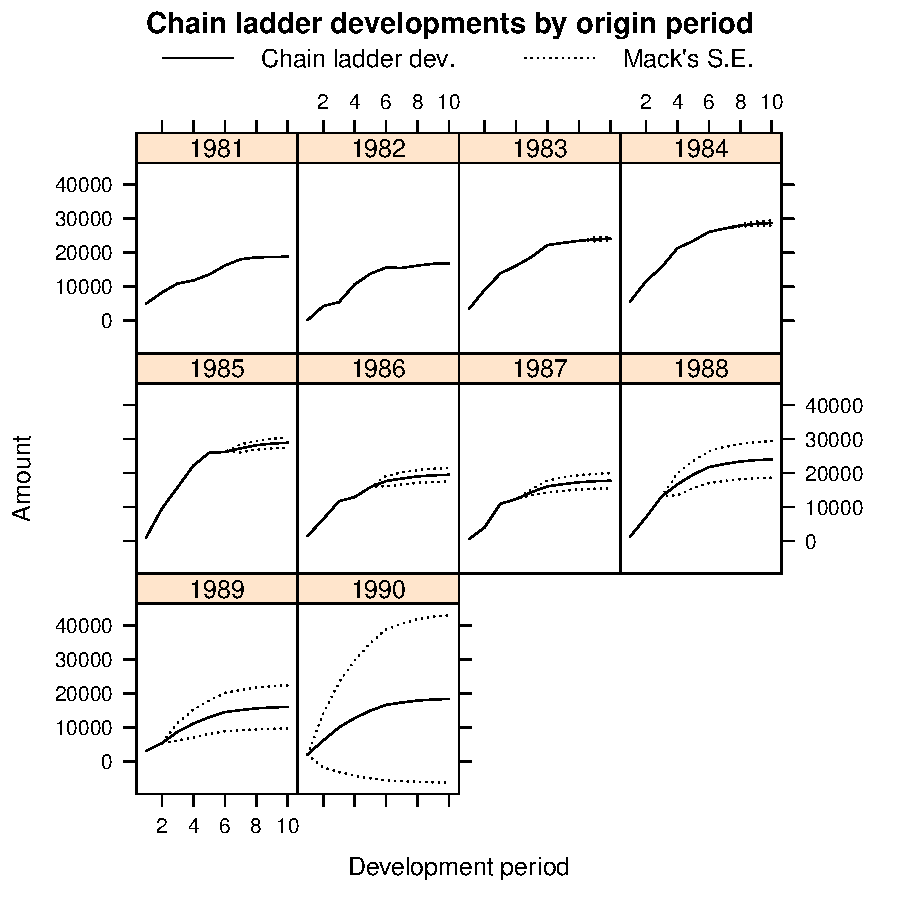
\includegraphics{ChainLadder-MackPlot2}
\end{center}

\subsubsection{Bootstrap chain-ladder}
\begin{Schunk}
\begin{Sinput}
R> # See also the example in section 8 of England & Verrall (2002) on page 55.
R> 
R> B <- BootChainLadder(RAA, R=999, process.distr="gamma")
R> B
\end{Sinput}
\begin{Soutput}
BootChainLadder(Triangle = RAA, R = 999, process.distr = "gamma")

     Latest Mean Ultimate Mean IBNR SD IBNR IBNR 75% IBNR 95%
1981 18,834        18,834         0       0        0        0
1982 16,704        16,875       171     740      200    1,369
1983 23,466        24,056       590   1,167      975    2,773
1984 27,067        28,740     1,673   1,829    2,552    5,134
1985 26,180        28,972     2,792   2,336    4,059    7,199
1986 15,852        19,557     3,705   2,481    5,088    8,154
1987 12,314        17,973     5,659   3,216    7,608   11,644
1988 13,112        24,367    11,255   5,054   14,359   20,674
1989  5,395        16,258    10,863   5,965   14,962   21,734
1990  2,063        19,288    17,225  14,125   23,713   42,761

                 Totals
Latest:         160,987
Mean Ultimate:  214,920
Mean IBNR:       53,933
SD IBNR:         18,726
Total IBNR 75%:  65,024
Total IBNR 95%:  85,721
\end{Soutput}
\begin{Sinput}
R> plot(B)
R> # Compare to MackChainLadder
R> MackChainLadder(RAA)
\end{Sinput}
\begin{Soutput}
MackChainLadder(Triangle = RAA)

     Latest Dev.To.Date Ultimate   IBNR Mack.S.E CV(IBNR)
1981 18,834       1.000   18,834      0        0      NaN
1982 16,704       0.991   16,858    154      143    0.928
1983 23,466       0.974   24,083    617      592    0.959
1984 27,067       0.943   28,703  1,636      713    0.436
1985 26,180       0.905   28,927  2,747    1,452    0.529
1986 15,852       0.813   19,501  3,649    1,995    0.547
1987 12,314       0.694   17,749  5,435    2,204    0.405
1988 13,112       0.546   24,019 10,907    5,354    0.491
1989  5,395       0.336   16,045 10,650    6,332    0.595
1990  2,063       0.112   18,402 16,339   24,566    1.503

               Totals
Latest:    160,987.00
Dev:             0.76
Ultimate:  213,122.23
IBNR:       52,135.23
Mack S.E.:  26,880.74
CV(IBNR):        0.52
\end{Soutput}
\begin{Sinput}
R> quantile(B, c(0.75,0.95,0.99, 0.995))
\end{Sinput}
\begin{Soutput}
$ByOrigin
     IBNR 75% IBNR 95% IBNR 99% IBNR 99.5%
1981      0.0        0        0          0
1982    199.8     1369     3120       4057
1983    974.8     2773     4613       5171
1984   2551.5     5134     7454       8285
1985   4059.1     7199    10194      11055
1986   5087.7     8154    11129      12396
1987   7607.6    11644    14316      16743
1988  14359.5    20674    25992      26549
1989  14962.5    21734    27153      29470
1990  23712.9    42761    60874      80560

$Totals
            Totals
IBNR 75%:    65024
IBNR 95%:    85721
IBNR 99%:   103434
IBNR 99.5%: 112226
\end{Soutput}
\begin{Sinput}
R> # fit a distribution to the IBNR
R> library(MASS)
R> plot(ecdf(B$IBNR.Totals))
R> # fit a log-normal distribution 
R> fit <- fitdistr(B$IBNR.Totals[B$IBNR.Totals>0], "lognormal")
R> fit
\end{Sinput}
\begin{Soutput}
    meanlog      sdlog  
  10.830859    0.373836 
 ( 0.011828) ( 0.008363)
\end{Soutput}
\begin{Sinput}
R> curve(plnorm(x,fit$estimate["meanlog"], fit$estimate["sdlog"]), col="red", add=TRUE)
R> 
\end{Sinput}
\end{Schunk}
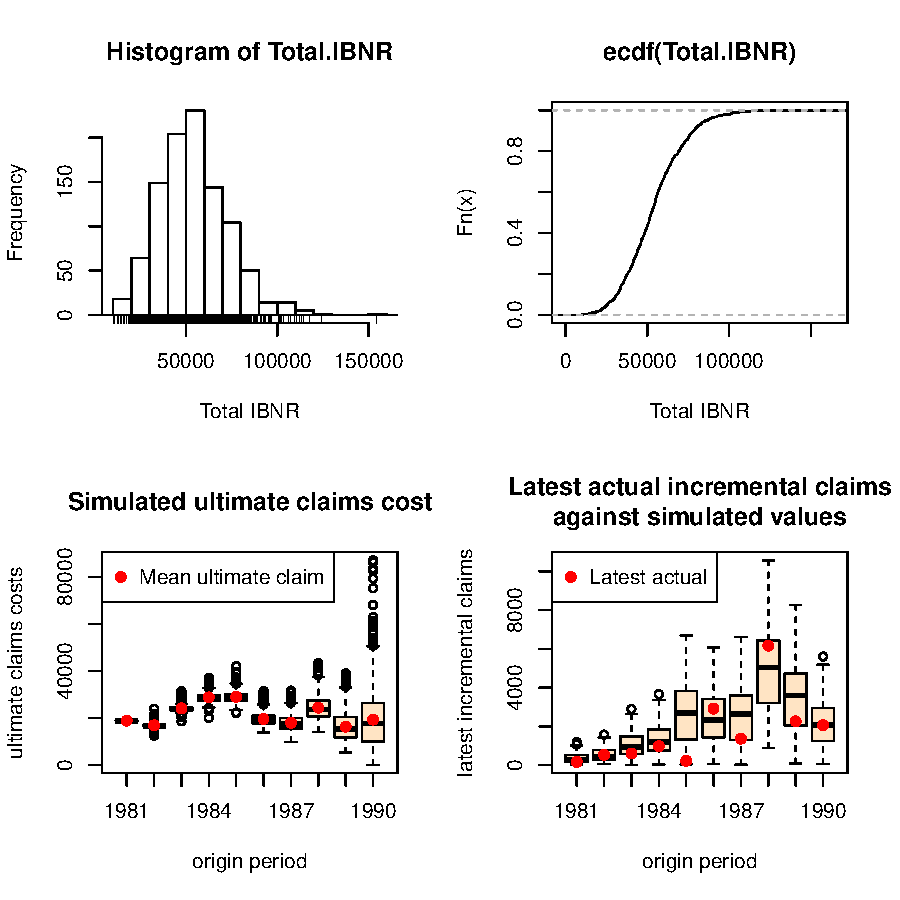
\includegraphics{ChainLadder-028}
\subsubsection{Munich chain-ladder}
\begin{Schunk}
\begin{Sinput}
R> MCLpaid
\end{Sinput}
\begin{Soutput}
      dev
origin    1    2    3    4    5    6    7
     1  576 1804 1970 2024 2074 2102 2131
     2  866 1948 2162 2232 2284 2348   NA
     3 1412 3758 4252 4416 4494   NA   NA
     4 2286 5292 5724 5850   NA   NA   NA
     5 1868 3778 4648   NA   NA   NA   NA
     6 1442 4010   NA   NA   NA   NA   NA
     7 2044   NA   NA   NA   NA   NA   NA
\end{Soutput}
\begin{Sinput}
R> MCLincurred
\end{Sinput}
\begin{Soutput}
      dev
origin    1    2    3    4    5    6    7
     1  978 2104 2134 2144 2174 2182 2174
     2 1844 2552 2466 2480 2508 2454   NA
     3 2904 4354 4698 4600 4644   NA   NA
     4 3502 5958 6070 6142   NA   NA   NA
     5 2812 4882 4852   NA   NA   NA   NA
     6 2642 4406   NA   NA   NA   NA   NA
     7 5022   NA   NA   NA   NA   NA   NA
\end{Soutput}
\begin{Sinput}
R> op <- par(mfrow=c(1,2))
R> plot(MCLpaid)
R> plot(MCLincurred)
R> par(op)
R> # Following the example in Quarg's (2004) paper:
R> MCL <- MunichChainLadder(MCLpaid, MCLincurred, est.sigmaP=0.1, est.sigmaI=0.1)
R> MCL
\end{Sinput}
\begin{Soutput}
MunichChainLadder(Paid = MCLpaid, Incurred = MCLincurred, est.sigmaP = 0.1, 
    est.sigmaI = 0.1)

  Latest Paid Latest Incurred Latest P/I Ratio Ult. Paid Ult. Incurred
1       2,131           2,174            0.980     2,131         2,174
2       2,348           2,454            0.957     2,383         2,444
3       4,494           4,644            0.968     4,597         4,629
4       5,850           6,142            0.952     6,119         6,176
5       4,648           4,852            0.958     4,937         4,950
6       4,010           4,406            0.910     4,656         4,665
7       2,044           5,022            0.407     7,549         7,650
  Ult. P/I Ratio
1          0.980
2          0.975
3          0.993
4          0.991
5          0.997
6          0.998
7          0.987

Totals
            Paid Incurred P/I Ratio
Latest:   25,525   29,694      0.86
Ultimate: 32,371   32,688      0.99
\end{Soutput}
\begin{Sinput}
R> plot(MCL)
\end{Sinput}
\end{Schunk}
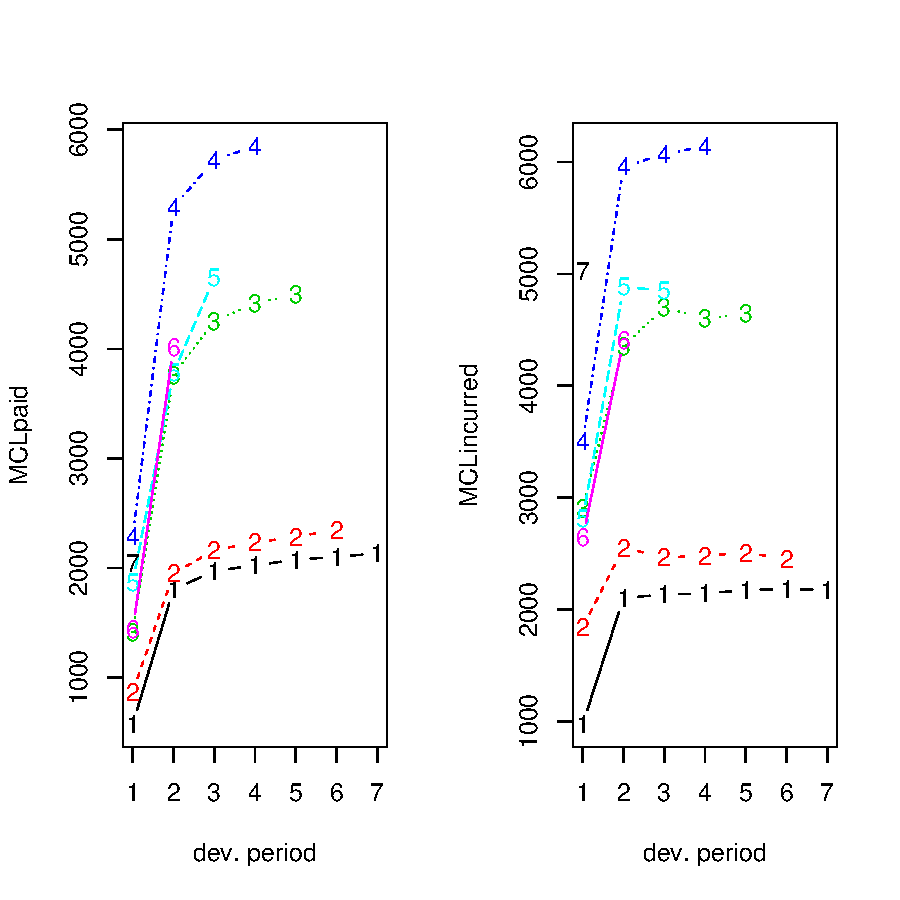
\includegraphics{ChainLadder-029}


\subsection{Multivariate chain-ladder}

\subsection{Clark's methods}

\subsubsection{Clark's Cap Cod method}

\subsubsection{Clark's LDF method}


\subsection{Generalised linear model methods}

%% \section{Using \chainladder with RExcel and SWord}

\section{Further resources}

Other useful documents and resources to get started with R in the
context of actuarial work:
\begin{itemize}
\item  Introduction to R for Actuaries~\cite{DeSilva2006}.

\item An Actuarial Toolkit~\cite{MaynardDeSilvaHollowayGesmannLauHarnett2006}.  

\item Actuar package vignettes: \url{http://cran.r-project.org/web/packages/actuar/index.html}
  
\item
  Mailing list
  \href{https://stat.ethz.ch/mailman/listinfo/r-sig-insurance}{R-SIG-insurance\footnote{\url{https://stat.ethz.ch/mailman/listinfo/r-sig-insurance}}}:
  Special Interest Group on using R in actuarial science and  insurance 
\end{itemize}




\subsection{Other insurance related R packages}

Below is a list of further R packages in the context of insurance. 
The list is by no-means complete, and the CRAN Task Views
\href{http://cran.r-project.org/web/views/Finance.html}{\emph{'Emperical
    Finance'}} and
\href{http://cran.r-project.org/web/views/Distributions.html}{\emph{Probability
    Distributions}} will provide links to additional resources. Please
feel free to contact \href{mailto:markus.gesmann@gmail.com}{us} with
items to be added to the list.

\begin{itemize}
\item \textbf{\texttt{cplm}}:  Monte Carlo EM algorithms and Bayesian methods for
  fitting Tweedie compound Poisson linear models~\cite{Zhang2011}.  
  
\item \textbf{\texttt{lossDev}}:  A Bayesian time series loss development
  model. Features include skewed-t distribution with time-varying
  scale parameter, Reversible Jump MCMC for determining the functional
  form of the consumption path, and a structural break in this
  path~\cite{LawsSchmid2011}. 
  
\item \textbf{\texttt{favir}}: Formatted Actuarial Vignettes in R. FAViR lowers the learning
  curve of the R environment. It is a series of peer-reviewed Sweave
  papers that use a consistent style~\cite{Escoto2011}. 
  
\item \textbf{\texttt{actuar}}: Loss distributions modelling, risk theory (including
  ruin theory), simulation of compound hierarchical models and
  credibility theory~\cite{DutangGouletPigeon2008}. 
  
\item \textbf{\texttt{fitdistrplus}}: Help to fit of a parametric distribution to
  non-censored or censored
  data~\cite{Delignette-MullerPouillotDenisDutang2011}.  

\item \textbf{\texttt{mondate}}: R packackge to keep track of dates in terms of
  months~\cite{Murphy2011}. 

\item \textbf{\texttt{lifecontingencies}}: Package to perform actuarial evaluation of
  life contingencies~\cite{Spedicato2011}. 
  
\end{itemize} 


\subsection{Presentations}
Over the years the contributors of the \chainladder package have given
numerous presentations and most of those are still available online:

\begin{itemize}

\item 
  \href{http://www.actuaryzhang.com/seminar/seminar.html}{Bayesian
    Hierarchical Models in Property-Casualty Insurance}, Wayne Zhang, 2011

\item
  \href{http://chainladder.googlecode.com/files/ChainLadder_Markus_20010Nov10.pdf}{ChainLadder
    at the Predictive Modelling Seminar, Institute of Actuaries,
    November 2010}, Markus Gesmann, 2011

\item
  \href{http://chainladder.googlecode.com/files/CAS-Spring-Meeting-2010-C21.pdf}{Reserve
    variability calculations},  CAS spring meeting, San Diego,
   Jimmy Curcio Jr., Markus Gesmann and Wayne Zhang,  2010

\item
  \href{http://chainladder.googlecode.com/files/ChainLadder_Markus_20090724.pdf}{The
    ChainLadder package, working with databases and MS Office
    interfaces, presentation at the "R you ready?" workshop} , Institute
  of Actuaries, Markus Gesmann, 2009
  
\item
  \href{http://chainladder.googlecode.com/files/ChainLadder_at_London_R_User_Group_20090331.pdf}
  {The ChainLadder package}, London R user group meeting, Markus
  Gesmann, 2009 

\item 
  \href{http://chainladder.googlecode.com/files/Introduction_to_R_20081203.pdf}{Introduction
    to R},
  \href{http://chainladder.googlecode.com/files/Loss_Reserving_in_R_20081203.pdf}{Loss
    Reserving with R},  Stochastic Reserving and Modelling Seminar, Institute of Actuaries,
  Markus Gesmann, 2008
  
\item
  \href{http://chainladder.googlecode.com/files/LossReserving%20with%20R%2020081113.pdf}{Loss
    Reserving with R} , CAS meeting, Vincent Goulet, Markus Gesmann and Daniel Murphy, 2008 
    
\item 
  \href{http://chainladder.googlecode.com/files/ChainLadderPackage_Dortmund_2008.pdf}{The
    ChainLadder package} R-user conference Dortmund, Markus Gesmann,
  2008
\end{itemize}

\subsection{Further reading}
Other papers and presentation which cited \chainladder:
\cite{Orr2007}, \cite{Nichols2009}, \cite{Zhang2010a},
\cite{MariaDoloresMartinezMiranda2010}, \cite{Schirmacher2010},
\cite{MariaDoloresMartinezMiranda2011}, \cite{Escoto2011},
\cite{Spedicato2011} 

\section{Training and consultancy}
Please contact \href{mailto:markus.gesmann@gmail.com}{us} if you would
like to discuss tailored training or consultancy.

\bibliographystyle{alpha}
\bibliography{ChainLadder}
\addcontentsline{toc}{section}{References} 

\clearpage

\section*{Thanks}
Many thanks to all who provided ideas, suggestions, 
corrections and bug reports:
\begin{itemize}
\item Nigel de Silva for all the ideas on how to use arrays effiecently
\item Florian Leitenstorfer for a bug report on MackChainLadder
\item Beat Huggler for comments on MunichChainLadder
\item Daniel Murphy for comments on MackChainLadder
\item Mark Hoffmann for a bug report on MackChainLadder
\item Christophe Dutang for ideas and code on utility functions to deal with triangles
\item Stefan Pohl for comments on tail factors with MunichChainLadder
\item Ben Escoto for providing a patch to a bug on returning latest incomplete triangle positions
\item Przemyslaw Sloma for reporting a bug in MackChainLadder
\item Ernesto Schirmacher for reporting a bug in residuals.MackChainLadder\end{itemize}
\end{document}
